\section{Ansible}
Ansible là một giải pháp đơn giản được sử dụng trong việc tự động hóa hàng loạt các công việc liên quan đến hạ tầng CNTT như tự động cấu hình, tự động triển khai phần mềm, và nhiều công việc khác nữa. Trong mô hình của Ansible, hạ tầng CNTT của bạn được nhìn góc độ là một kiến trúc tổng thể của các thành phần có liên quan thay vì chỉ quản lý một hệ thống tại một điểm riêng lẻ. Nó không sử dụng các agent hoặc thêm vào các lớp tùy chọn bảo mật bổ sung, do đó việc triển khai Ansible vô cùng đơn giản. Một điều quan trọng nữa đó là ngôn ngữ cấu hình mà nó sử dụng rất đơn giản (được gọi là playbooks), nó cho phép mô tả những công việc tự động bằng tiếng Anh đơn thuần thay vì viết một điều gì đó phức tạp bằng một ngôn ngữ lập trình nào đó. Bằng cách sử dụng Ansible, chúng ta sẽ thực hiện việc tự động hóa hàng loạt nhanh hơn, thậm chí nó có thể đạt tới những điều mà ta chưa từng thấy trước đó.

\subsection{Tổng quan}

Ansible là một phần mềm mã nguồn mở dùng trong việc quản lý cấu hình của hạ tầng CNTT, triển khai sản phẩm công nghệ, cùng như điều phối các hoạt động tự động hóa khác. Với chỉ một công cụ duy nhất, nó đem lại những hiệu quả lớn trước hàng loạt các thách thức về tự động hóa. Ansible cung cấp sự thay thế hiệu các chức năng cốt lỗi vốn có trong các giải pháp tự động hóa khác, đồng thời tìm kiếm lời giải cho những vấn đề chưa được giải quyết. Bao gồm sự phối hợp rõ ràng về các quy trình làm việc phức tạp và sự thống nhất về cấu hình của hệ điều hành và phần mềm ứng dụng triển khai.

\newpage
\clearpage

Ansible tìm cách giữ cho những mô tả về các quy trình công việc dễ hiểu và có thể được thực hiện nhanh chóng. Điều đó đồng nghĩa với việc những người mới sử dụng Ansible có thể nhanh chóng hòa nhập vào các dự án mới, đồng thời dễ dàng hiểu được những công việc cho dù họ có tham gia vào dự án muộn hơn. Không chỉ vậy, Ansible luôn tìm cách tạo ra những công cụ thật mạnh mẽ cho những chuyên gia, nhưng bình đẳng cho tất cả các cấp độ kỹ năng của người sử dụng. Từ đó, rút ngắn thời gian đưa sản phẩm ra thị trường; giảm thiểu các lỗi có thể xảy ra do sự thay đổi cấu hình của hạ tầng CNTT.

Ansible được thiết kế nhỏ gọn, tiện dụng, an toàn, và có độ tin cậy cao, không mất nhiều công sức trong việc học sử dụng cho dù là quản trị viên, nhà phát triển hay nhà quản lý.

\subsection{Kiến trúc hệ thống}

\begin{figure}[h!]
    \begin{center}
    \fbox{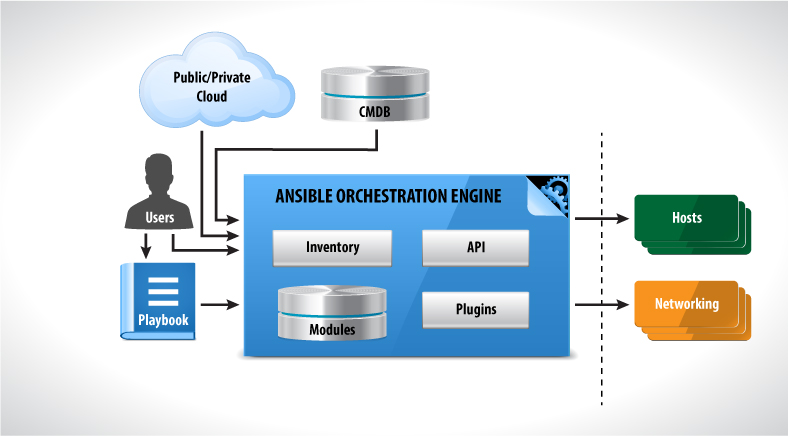
\includegraphics[width=\textwidth]{images/ansible_architect.jpg}}
    \end{center}
    \caption{Kiến trúc hệ thống của Ansible}
    \label{fig:ansible_arch}
\end{figure}

\newpage
\clearpage

Một trong những khác biệt chính giữa Ansible với những sản phẩm cùng loại chính là kiến trúc của nó

\begin{itemize}
\item Mặc định, Ansible quản lý các máy trạm thông qua giao thức SSH. Nó sử dụng một thư viện được gọi là \textbf{paramiko} (được viết bằng lập trình Python\footnote{\url{https://en.wikipedia.org/wiki/Python_(programming_language)}}) hoặc sử dụng ngay OpenSSH của hệ điều hành.

\item Ansible có thể truyền tải theo khác nhau, các phương thức là có thể thay đổi được. Ví dụ: Mặc dù \textbf{0mq} - một phương thức truyền tải tăng tốc (accelerated transport) được đưa ra nhưng Ansible hỗ trợ cả phương thức không sử dụng mạng.

\item Ansible không yêu cầu quyền root\footnote{account có quyền tuyệt đối với hệ thống trên Linux, BSD hay Solaris} để truy cập mà nó có thể cấu hình để dùng sudo\footnote{\url{https://en.wikipedia.org/wiki/Sudo}} trong các trường hợp cần thiết.

\item Ansible không yêu cầu một khóa SSH cụ thể hay một người dùng riêng. Nó có thể làm việc với bất cứ người sử dụng được cung cấp, nghĩa là Ansible tôn trọng quyền truy cập của hệ điều hành của bạn.

\item Khi có yêu cầu, Ansible sẽ chuyển các module cần thiết tới các nút điều khiển, sau đó chạy chúng từ xa với các thông tin người dùng đã được cung cấp và không để lại được bất cứ cài đặt gì trên các nút này.

\item Ansible không yêu cầu bất kỳ phần mềm máy chủ được chạy từ một máy quản lý, nó chỉ yêu cầu các thông tin đăng nhập của người dùng mà thôi.

\item Ansible không yêu cầu bất kì một phần mềm agent nào được chạy trên cái nút điều khiển.

\item Ansible không cần mở thêm bất cứ một cổng nào ngoài SSH cũng như không yêu cầu phải có hạ tầng PKI để bảo trì.

\item Những người có quyền truy cập vào máy chủ điều khiển (hoặc máy chủ điều khiển mã nguồn) không thể xóa hay thay đổi các nội dung các máy trạm (hoặc ra lệnh cho chúng chạy một lệnh nào đó) mà không có cũng có thông tin về hệ thống đó.

\item Khi không còn quản lý nữa, Ansible không dùng đến bất cứ tài nguyên nào của những máy trạm.

\end{itemize}

Những đặc điểm trên kết hợp với nhau làm cho Ansible trở nên lý tưởng cho các môi trường bảo mật hoặc hiệu suất cao, nơi có những lo ngại về sự ổn định hoặc việc thay đổi thường xuyên của các agent. Những thuộc tính trên hầu hết đều hữu ích trong các lĩnh vực về máy tính.

Ansible là sự thiết kế đồng nhất giữa kinh nghiệm của sử dụng và phương pháp tiếp cận. Ansible được thiết kế để làm cho việc cấu hình và xử lý các hạ tầng CNTT cũng chỉ đơn giản như việc đọc hoặc viết cấu hình, thậm chí đối với những người chưa qua đào tạo về việc đọc chúng.

Mặc dù Ansible có thể thực hiện hầu hết các loại nhiệm vụ tự động hóa, Ansible không giống với ngôn ngữ lập trình phần mềm, nó chỉ là các mô tả cơ bản về trạng và tiến trình. Hơn nữa, nó cố gắng để giải quyết nhiều vấn đề chồng chéo của tự động hóa hệ thống từ một framework duy nhất với mục tiêu giảm thiểu thời gian và chi phí để học và hiểu cũng như gắn kết nhiều framework với nhau.

Với các phương pháp truyền thống khác, người dùng thường phải kết hợp nhiều công cụ với nhau có để bao quát hết những điều cơ bản trong quản lý hệ thống CNTT và cấu hình phần mềm, bao gồm:

\begin{itemize}
\item Một công cụ dùng quản lý cấu hình, nó dùng để làm việc với các hệ điều hành cơ bản, mô tả các trạng thái mong muốn của một hệ thống, nhưng không phải quá trình để đưa nó vào trạng thái đó.

\item Một công cụ triển khai, dùng để đưa sản phẩm phần mềm lên hệ thống, nó tập trung vào quá trình thực hiện.

\item Một công cụ dùng để thực thi, cho các tác vụ thực thi tức thời - những thứ mà không phù hợp với mô hình trước đây, chẳng hạn như restart hàng loạt các máy chủ.
\end{itemize}

Ansible đã gộp tất cả các yếu tó đó thành một công cụ duy nhất, đồng thời cung cấp các khả năng và đặc điểm cho phép thực hiện triển khai những phần mềm nhiều lớp và các quy trình làm việc phức tạp.

\subsection{Mô hình sắp xếp công việc}

Để có thể hiểu được mô hình sắp xếp công việc (Modeling Orchestration Workflows) của Ansible, chúng ta lấy xem xét một ví dụ cụ thể về một ứng dụng web 3 lớp truyền thống bao gồm các thành phần:

\begin{itemize}
\item Các máy chủ ứng dụng
\item Các máy chủ cơ sở dữ liệu
\item Các máy chủ nội dung
\item Hệ thống cân bằng tải
\item Hệ thống giám sát được kết nối với hệ thống cảnh báo như một dịch vụ thông báo
\item Một hệ thống tích hợp liên tục\footnote{Continuous integration: \url{https://en.wikipedia.org/wiki/Continuous_integration}}
\end{itemize}

Theo như ví dụ trên, Ansible có thể xử lý một cách đơn giản theo mô hình như sau:

\begin{enumerate}
\item Tư vấn cách cấu hình và cài đặt kho chứa cho thông tin về các máy chủ tham gia.
\item Cấu hình hệ điều hành cơ sở trên tất cả các máy và thực hiện các công việc sao cho tất cả chúng có cùng một trạng thái mong muốn.
\item Xác định thành phần của các máy chủ ứng dụng web để cập nhật.
\item Đưa ra tín hiệu báo cho hệ thống giám sát chuyển các servers vào trạng thái offline.
\item Đưa ra tín hiệu báo cho hệ thống cân bằng tải tách các máy chủ ứng dụng ra khỏi hệ thống
\item Triển khai và cập nhật các máy chủ ứng dụng web
\item Đưa ra tín hiệu báo cho hệ thống cân bằng tải đưa các máy chủ ứng dụng này trở lại hệ thống.
\item Đưa ra tín hiệu báo cho hệ thống giám sát tiếp tục giám sát các sự cố trên các máy chủ này.
\item Lặp đi lặp lại quá trình này cho tới khi tất cả các máy chủ ứng dụng còn lại được cập nhật.
\item Lặp lại các quá trình cập nhật lần lượt này cho các lớp khác như máy chủ cơ sở dữ liệu hay máy chủ nội dung.
\item Gửi thư điện thử thông báo và giải trình khi quá trình cập nhật hoàn thành.
\end{enumerate}

\subsection{Các thành phần chính}

\subsubsection{Modules}


Các module của Ansible là nguồn tài nguyên được phân phối cho các nút ở xa để yêu cầu chúng thực hiện một số nhiệm vụ hoặc đưa nút đó một vào một trạng thái thích hợp theo yêu cầu. Ansible luôn đi theo triết lý "batteries included", vì vậy chúng ta có rất nhiều module tuyệt vời dành cho hầu hết các công việc lõi của ngành CNTT. Điều này có nghĩa là những module này luôn được cập nhật và chúng ta không cần phải cố gắng tìm kiếm cách để cho nó làm việc trên nền tảng của chúng ta. Chúng ta có thể tưởng tượng những module này là các thành phần của một bộ công cụ hữu ích với các công cụ quản lý hệ thống và các playbooks như một hướng dẫn để xây dựng một hệ thống bằng những công cụ này.

Với một số lượng khá lớn module, Ansible có khả năng dễ dàng triển khai những workloads tới một loạt các công nghệ ảo hóa và các dịch điện toán đám mây công cộng hay trên các môi trường tiền điện toán đám mây như VMware, OpenStack, Amazon Web Services EC2 (AWS), Eucalyptus Cloud, KVM, và CloudStack. Những máy chủ có thể được triển khai từ hình ảnh hệ điều hành cơ sở mà không có bất kỳ sửa đổi, đồng thời được cấu hình đầy đủ chỉ trong một bước.

Không chỉ vậy, hiện nay Ansible được sử dụng rộng rãi trong việc triển khai các hệ thống BigData, các hệ thống lưu trữ và phân tích môi trường bao gồm những nền tảng quan trọng như Hadoop, Riak, và Aerospike.

Trong những môi trường có nhiều máy chủ chưa được cấu hình nhưng chúng phải được cấu hình trước mà không cần bất kì một chương trình agent quản lý. Khách hàng yêu cầu một công cụ điều khiển đơn giản và dễ dàng chỉnh sửa các chính sách cho cả hai việc triển khai và cập nhật các cụm clusters.

Các khu vực khác bên ngoài lĩnh vực BigData cũng có thể tận dụng lợi thế này. Các tính chất này cũng làm cho Ansible hấp dẫn cho hệ thống giám sát lưu lượng truy cập cao tổ chức, nơi Ansible trả lại tất cả tài nguyên CPU có sẵn cho các môi trường máy tính khi không sử dụng. Không có việc lãng phí tài nguyên bộ nhớ hoặc CPU, cũng không cần phải có một daemon để duy trì hoạt động.

Để có thể tìm hiểu chi tiết hơn về chức năng của các module này trong Ansible, chúng ta có thể tham khảo trang tài liệu của Ansible Works. Tại địa chỉ \url{http://www.ansibleworks.com/docs/modules.html}

\subsubsection{Plugins}

Có rất nhiều điểm tích hợp có thể được sử dụng để mở rộng Ansible, bao gồm:

\begin{itemize}
\item Những module có thể chạy cục bộ hoặc từ xa để cấu hình các ứng dụng, các dịch vụ hoặc các tham số cho hệ điều hành.
\item Các phương thức mới ghi nhập các callback cho các chương trình kiểm soát hoặc báo cáo
\item Tích hợp với các nguồn dữ liệu bên ngoài
\item Các thông tin dữ liệu của Inventory từ hệ thống CMDB hoặc đám mây
\item Các phương thức chuyển vận mới mà từ đó Ansible có thể giao tiếp với các máy mà mình quản lý
\end{itemize}

Các đơn vị công việc trong ansible được đảm bảo bởi các module, đó là những chương trình nhỏ chạy trên máy chủ ở xa để đảm bảo rằng máy chủ đó được đưa vào trạng thái chỉ định phù hợp. Các module này có thể viết bằng ngôn ngữ bất kì chẳng hạn như Python, Perl, Ruby hay bash script. Vì vậy, người dùng có thể sử dụng công cụ yêu thích của họ để tạo ra các module cho bản thân mình hay những người khác.

Mặc định, các module lõi đã được tạo sẵn, có nghĩa là chúng giúp hệ thống có được một trạng thái mong muốn, và nếu không có thay đổi trạng thái được thực hiện, chúng không làm gì ảnh hưởng tới hệ thống cả. Ansible cũng làm cho nó trở nên dễ dàng để mô hình hóa các quá trình được không tạo sẵn, và cũng làm cho nó có thể chỉ đơn giản là chỉ cần đẩy ra kịch bản đơn giản và chạy chúng như mong muốn. Sử dụng các module có sẵn là thích hơn, tuy nhiên, nhưng điều quan trọng hơn là có thể mô hình hóa bất kỳ loại quá trình nào chứ không chỉ một và rơi vào những giới hạn của chúng. Ansible luôn thực tế trong vấn đề này.


\subsubsection{Playbook}


Trong Ansible, mọi công việc từ cấu hình hệ điều hành cơ sở đến mô hình hóa quá trình cập nhật hay thực thi ngay lập tức các công việc trên một máy chủ ở xa đều sử dụng chung một công cụ. Những cấu hình cụ thể được viết ra trong Ansible được gọi là "Playbook". Đó một dạng mã mà cả con người và máy tính đều có thể phân tích được (một dạng mã YAML\footnote{\url{http://www.ansibleworks.com/docs/YAMLSyntax.html}}), đồng thời làm cho việc hợp tác với những chương trình khác dễ dàng hơn. Và quan trọng nhất là dễ đọc và hiểu đối với cả những người không phải là nhà phát triển.

Playbook làm cho việc cấu hình hệ thống hay triển khai hệ thống trên nhiều máy trở lên đơn giản hơn bất kỳ công cụ nào đã có. Playbook rất phù hợp trong việc triển khai các ứng dụng phức tạp.

Playbook có thể khai báo cấu hình, nhưng nó cũng có thể dàn xếp các bước bất kì của một quá trình thủ công, thậm chí là cả những bước khác nhau khi mà chúng phải nhảy qua nhảy lại giữa một tập hợp các máy chủ với các nhiệm vụ khác nhau. Playbook có thể thực hiện các công việc một cách đồng bộ hoặc không đồng bộ.

Trong khi bạn có thể chạy chính Ansible cho các nhiệm vụ đột xuất, playbook có thể được giữ trong các hệ thống kiểm soát mã nguồn và được sử dụng để đẩy đi các cấu hình hoặc đảm bảo cấu hình của hệ thống từ xa được giữ trong spec của nó.

Playbook được thể hiện trong định dạng YAML với cú pháp được tối thiểu hóa. Những nhà phát triển Ansible đã hết sức cố gắng để làm cho nó không giống một ngôn ngữ lập trình hay script mà là giống một dạng mô hình cấu hình hay một quá trình.

Mỗi playbook bao gồm một hay nhiều \textbf{play} trong danh sách

Mục tiêu của mỗi play là ánh xạ một nhóm các máy chủ với một số vai trò xác định, đại điện cho những điều mà Ansible gọi là nhiệm vụ (task). Ở mức độ cơ bản, một nhiệm vụ không gì hơn là gọi đến một module của Ansible

Bằng cách gộp nhiều play, Playbooks có thể dàn xếp việc triển khai trên nhiều máy, chạy một số bước nhất định trên nhóm máy chủ web, sau đó một số khác trên nhóm máy cơ sở dữ liệu, sau đó lại là một nhóm lệnh khác trên các máy chủ web ... cứ vậy cho đến khi hoàn thành.

\begin{lstlisting}[label={lst:ansible_playbook_example},caption={Ví dụ về playbook của Ansible},morekeywords={hosts, vars, tasks, name, yum, http_port, max_clients, remote_user, template, service, handlers, notify, state, pkg, src, dest}]
- hosts: webservers
  vars:
    http_port: 80
    max_clients: 200
  remote_user: root
  tasks:
  - name: ensure apache is at the latest version
    yum: pkg=httpd state=latest
  - name: write the apache config file
    template: src=/srv/httpd.j2 dest=/etc/httpd.conf
    notify:
    - restart apache
  - name: ensure apache is running
    service: name=httpd state=started
  handlers:
    - name: restart apache
      service: name=httpd state=restarted
\end{lstlisting}

"play" ít hoặc nhiều có những nét tương đồng với những môn thể thao. Chúng ta có có thể có khá nhiều play ảnh hưởng đến hệ thống của chúng ta theo nhiều cách khác nhau. Điều đó nghĩa là nếu chúng ta định nghĩa ra một mô hình hoặc một trạng thái, chúng ta có thể chạy nhiều play khác nhau tại các thời điểm khác nhau.

Trong playbook trên, nó chỉ chứa duy nhất một play, chúng ta khai báo một cụm \textbf{webservers} ở cổng 80 và có số client tối đa là 200, sử dụng user root để điều khiển. Playbook cũng thiết lập một số công việc và trạng thái mong muốn với nó:

\begin{itemize}
\item Đảm bảo chắc chắn rằng Apache httpd server là phiên bản mới nhất
\item Đảm bảo config của Apache \textbf{/etc/httpd.conf} giống như template có sẵn ở \textbf{/srv/httpd.j2}. Đồng thời thiết lập thông báo khi Apache restart.
\item Đảm bảo rằng Apache đã được khởi động
\end{itemize}

\subsection{Cách cài đặt và sử dụng}

Ansible có thể cài đặt và chạy trên bất cứ máy tính nào có cài đặt Python 2.6. Hầu hết các nền tảng đều hỗ trợ mặc định Python trong hệ thống bao gồm cả RHEL, CentOS, Debian, Ubuntu hoặc bất cứ bản phân phối Linux nào hỗ trợ Python; Mac OS X, các hệ điều hành thuộc họ BSD ...

\subsubsection{Cách cài đặt Ansible trên máy điều khiển}

\textbf{• Cài đặt từ mã nguồn}

Ansible là rất dễ dàng để cài đặt từ mã nguồn, nó không yêu cầu sử dụng quyền root và cũng không có bất cứ phần mềm nào được sử dụng để cài Ansible ngoài chính nó. Không cần phải có daemon hoặc cơ sở dữ liệu nào cho việc cài đặt. Vì thế, nhiều người trong cộng đồng của Ansible luôn sử dụng phiên bản đang được phát triển để họ có thể tận dụng lợi thế của các tính năng mới khi chúng đang được thực hiện, và cũng dễ dàng đóng góp vào dự án. Đi theo các phiên bản đang phát triển luôn là cách nhanh và dễ dàng nhất để theo đuổi một dự án phần mềm nguồn mở.


\begin{lstlisting}[label={lst:ansible_install_from_source},caption={Cài đặt Ansible từ mã nguồn}, language=bash, deletekeywords={env}]
$ git clone git://github.com/ansible/ansible.git
$ cd ./ansible
$ source ./hacking/env-setup
\end{lstlisting}

Nếu máy điều khiển chưa được cài đặt \textbf{pip} thì chúng ta cần phải cài đặt pip, sau đó cài thêm một số moudule python cần thiết cho Ansible

\begin{lstlisting}[label={lst:ansible_install_module_pip},caption={Cài đặt các module cần thiết cho Ansible bằng pip}, language=bash, deletekeywords={}]
# Install pip tool
$ sudo easy_install pip
# Install python modules
$ sudo pip install paramiko PyYAML jinja2 httplib2
\end{lstlisting}

\textbf{• Cài đặt thông qua Yum trên RHEL, CentOS}

Ansible luôn có sẵn trong kho phần mềm EPEL\footnote{\url{https://fedoraproject.org/wiki/EPEL}} 6 của Fedora, tuy nhiên các dòng sử dụng trình quản lý gói rpm đều có thể sử dụng được.

Ansible có thể chạy được trên cả các phiên bản trước đó EL5 chứa Python 2.4 hoặc cao hơn.

\begin{lstlisting}[label={lst:ansible_install_yum},caption={Cài đặt Ansible từ mã nguồn}, language=bash, deletekeywords={}]
# Install EPEL repo
$ rpm -ivh https://dl.fedoraproject.org/pub/epel/6/x86_64/epel-release-6-8.noarch.rpm
# Install ansible with dependencies modules
$ sudo yum install ansible
\end{lstlisting}

Chúng ta cũng có thể tự build gói rpm cho chính mình. Từ thư mục chủ của mã nguồn Ansible, chúng ta gõ lệnh \textbf{make rpm} để build gói rpm mà chúng ta có thể cài đặt bằng yum; để build được bạn cần cần cái gói \textbf{\textit{rpm-build}}, \textbf{\textit{make}}, \textbf{\textit{python2-devel}}.

\begin{lstlisting}[label={lst:ansible_install_build_rpm},caption={Tự build gói rpm của Ansible}, language=bash, deletekeywords={}]
$ git clone git://github.com/ansible/ansible.git
$ cd ./ansible
$ make rpm
$ sudo rpm -Uvh ~/rpmbuild/ansible-*.noarch.rpm
\end{lstlisting}

\textbf{• Cài đặt thông qua Apt trên Debian, Ubuntu}

Với distro Ubuntu, Ansible có thể được cài đặt thông qua hệ thống PPA\footnote{https://launchpad.net/~rquillo/+archive/ansible} theo các bước sau:

\begin{lstlisting}[label={lst:ansible_install_ppa},caption={Cài đặt Ansible trên Ubuntu thông qua PPA}, language=bash, deletekeywords={}]
$ sudo add-apt-repository ppa:rquillo/ansible
$ sudo apt-get update
$ sudo apt-get install ansible
\end{lstlisting}

\textbf{• Cài đặt thông qua pip}

Ansible cũng có thể cài đặt thông qua \textbf{pip} - Python package manager.

\begin{lstlisting}[label={lst:ansible_install_pip},caption={Cài đặt Ansible thông qua pip}, language=bash, deletekeywords={}]
# Install pip - python package manager
$ sudo easy_install pip
# Install Ansible
$ sudo pip install ansible
\end{lstlisting}

\subsubsection{Cấu hình và làm quen với Ansible}

Ở phía trên chúng ta đã tìm hiểu cách cài đặt Ansible thông qua một số cách thông dụng, trong phần này chúng ta sẽ tìm hiểu các cấu hình và một số thao tác cơ bản với Ansible.

Để có thể bắt đầu làm việc với cái máy cần điều khiển, chúng ta cần cấu hình các Inventory cho Ansible.

Các thông số về máy chủ cũng như các cụm máy chủ được Ansible lưu trữ ở \textbf{/etc/ansible/hosts} với format giống file ini.

\begin{lstlisting}[label={lst:ansible_config_inventory},caption={Cấu hình Inventory của Ansible}]
mail.example.com

[webservers]
foo.example.com
bar.example.com

[dbservers]
one.example.com
two.example.com
three.example.com
\end{lstlisting}

Chi tiết về cách cấu hình inventory, chúng ta có thể xem tại đây\footnote{\url{http://www.ansibleworks.com/docs/intro_inventory.html}}

Chúng ta có thể sử dụng Ansible để thao tác quản lý file trên máy chủ, quản lý các gói phần mềm, quản lý người dùng, quản lý các dịch vụ và triển khai các sản phẩm từ hệ thống quản lý mã nguồn ...

\begin{lstlisting}[label={lst:ansible_adhoc_command},caption={Ansible thực hiện các chức năng thông qua dòng lệnh}, language=bash, deletekeywords={}]
# File transfer
$ ansible atlanta -m copy -a "src=/etc/hosts dest=/tmp/hosts"
$ ansible webservers -m file -a "dest=/srv/foo/b.txt mode=600 owner=mdehaan group=mdehaan"

# Package Manager
$ ansible webservers -m yum -a "name=acme state=installed"
$ ansible webservers -m yum -a "name=acme state=removed"

# User & Group
$ ansible all -m user -a "name=foo password=<crypted password here>"
$ ansible all -m user -a "name=foo state=absent"

# Deploy from source control
$ ansible webservers -m git -a "repo=git://foo.example.org/repo.git dest=/srv/myapp version=HEAD"

# Services
$ ansible webservers -m service -a "name=httpd state=started"
$ ansible webservers -m service -a "name=httpd state=stopped"

\end{lstlisting}

Trên đây là một số làm quen cơ bản với Ansible, chúng ta có thể đọc thêm nhiều ví dụ hơn trong các tài liệu khác của Ansible trong các địa chỉ dưới đây:

\begin{itemize}
\item \url{http://www.ansibleworks.com/docs/playbooks_best_practices.html}
\item \url{http://www.ansibleworks.com/docs/modules.html}
\item \url{https://github.com/ansible/ansible-examples}
\end{itemize}


\subsection*{Tóm lại}

Ansible với một tập hợp của các công cụ đơn giản và gọn nhẹ nhưng đồng thời lại rất mạnh mẽ. Ansible có thể bao quát hết các vấn đề của tự động hóa. Việc học sử dụng hay cấu hình Ansible rất dễ dàng cho dù đối với cả những người chưa từng tiếp xúc với nó. Nó xứng đáng là một công cụ hàng đầu về tự động hóa cho các quản trị hệ thống.